The power and importance of graph structures is clearly eveident in the varied application of graphs in  drug design, protein structure comparison, video indexing, topology of sensor networks \cite{in_zang2011} and social and information networks\cite{in_williams2007} \cite{in_chen2007}. As a result a tremendous amount of structured data is being accumulated in large databases. An essential problem in managing the large amount of graphs and graph queries is the efficiency of query processing.

A graph database can  be viewed as either a large single graph(e.g. social network) or a collection of labelled graphs (protein database). Graph searching then refers to (sub)graph-to-graph matching in datagraphs\cite{sasha2002}. In general, two methods of (sub)graph-to-graph search have been used. The first is fast (sub)graph-to-graph search algorithms. Examples of these are \cite{ullmann1976}\cite{cordella2004_vf2}. More recentresearch has focused on the use of indexing techniques\cite{sasha2002} \cite{yan2005} \cite{he_singh2006} \cite{zhang2007} \cite{jiang2007} \cite{cheng2007} \cite{zhao2007} to close the speed gap with traditional text search. The use of indexing is attractive as a means to overcome the inherent exponential worst case complexity of graph search. The general view is that most indexing graph search is based on filter-and-verify methodology\cite{sasha}. Relatively few, highly discriminative features are selected to index a large graph database. When a query is given, the search space is reduced first by finding the most relevant graphs or, for a single graph database, most relevant subgraphs, using the feature index. Next the query is formulated into simple structures (set of nodes, edges or paths). And finally graph matching, the verification stage, which is implemented by either (sub)graph-to-graph matching techniques or by combining paths from path processing path expressions in the query, through the database. Verification is necessary because to speed up the fitering process, non graph techniques are used reduce candidate graphs.  


Classical graph matching can be viewed as the final, verification step in the indexed graph search. In its simplest form an enumeration algorithm to find occurences of a query graph $G_a$ in a data graph $G_b$ is to generate all possible maps between the nodes of the two graphs and then to verify if each generated map is a match. All maps can be represented using a \textit{state space representation} tree  where a node represents a match between a pair of vertices and a path from the root to the leaf represents a map between two graphs. Paths from the root to an intemediary level represent a partial match indicating that only a subset of the vertices have been matched. The complexity of such an enumeration algorithm is exponential and subgraph isomorphism is proven to be NP-complete\cite{garey_johnson1979_in_sasha2002(42)}.

There have been many attempts to reduce the cost of (sub)graph graph searching, by loosening the criteria by approximate algorithms\cite{sasha2002} which have polynomial complexity, but not guarantee to find the correct solution. Two further categories are exact and inexact (or error correcting) algorithms that are guaranteed to find the correct answer and have therefore exponential worst case complexity.

The most popular exact(and inexact) subgraph matching algorithms are based on heuristics on the state space representation tree that corresponds to a subisomorphism\cite{ullmann}. The performance of ullmann's  \textit{state-space representation  with backtracking} algoritm is improved by a refinement procedure called \textit{forward checking} where in order to insert a node  in the tree two conditions must be met. Submorphism must hold and a possible matching must exist for \textit{all} unmatched vertices. 


Largly uninvestigated is the problem of efficiently searching for (sub)graphs directly in large graph databases. But the But it is also an expression of the lack of more efficient algorithms. 




 has let to an increasingly in Graphs have become increasingly important structures for representing and understanding complex structures in a wide range of applications.
In computational biology, graph models of protein molecules are used to mine frequent substructural motifs\cite{Huan2005}. In chemical informatics, graphs are used to model the molecular structure of chemical compounds. Graphs are also used in diverse fields such as pattern recognition, computer vision, social networks and so on. Such applications require that graph queries are solved efficiently.

Deciding whether a graph contains another graph is called the \textit{subgraph isomorphism problem}. That is, a subgraph isomorphism exist between two graphs if there exists one-to-one mapping between the smaller graph and a subgraph of the larger graph such that edge the adjacencies are preserved. Testing for subgraph isomorphism for an $n$-node graph in an $m$-node larger graph is a combinatorial matching with $m^n$ possibilities, hence is expensive. Therefore for a given query, evaluating a database for subgraph  isomorphism by individually testing each graph  in the database is inefficient.  In fact, the subgraph isomorphism problem is known to be NP-complete\cite{np-complete}. In  many 
cases, the graph database is also very large. This makes it necessary to build a framework to facilitate efficient graph search.

%\begin{figure}
%\centering
%\epsfig{file=images/typical_subgraph_query.eps, height=2.5in, width=2.5in}
%\caption{Subgraph isomorphism query}
%\label{fig:fig101}
%\end{figure}


\begin{figure}
\centering
%& -shell-escape -enable-write18
\documentclass{standalone}
\usepackage{tikz}
\usetikzlibrary{external}
%\tikzexternalize
\usetikzlibrary{shapes,arrows}
\usepackage{caption}
\usetikzlibrary{matrix}
%\newcommand{mynodename}[#1]{\mathrm{#1}}\label{•} 
%\newcommand{mylabelleft}[#2]{label={[font=\fontsize{#1}{#1}\selectfont]above left:mynodename{#2}}}

\begin{document}
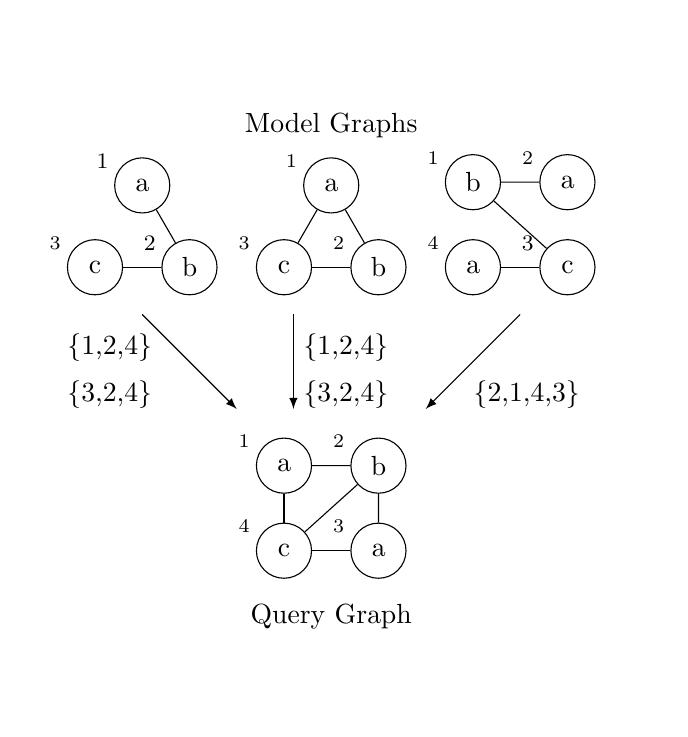
\begin{tikzpicture}[scale=1.2]
%[every node/.style={draw,circle}]
\tikzstyle{every node}=[draw,shape=circle,minimum size=0.7cm];
\tikzstyle{line} = [draw,-latex]
\colorlet{invisible}{white}
\colorlet{visible}{black}
%\tikzstyle{mylabelsfont=[font=\fontsize{7}{7}\selectfont,yshift=-.2cm];
%\tikzstyle{every label}=[text height=10pt];
\begin{scope}[shift={(0,-0.5)}] 
	\begin{scope}[yshift=0cm]% top row as a group
%	\draw[help lines] (-1,-6) grid (10,6);
	  \node (a) at (60:1cm) [label={[font=\fontsize{8}{8}\selectfont,yshift=-.2cm]above left:$1$}] {a};
	  \node (b) at (0:1cm)  [label={[font=\fontsize{8}{8}\selectfont,yshift=-.2cm]above left:$2$}] {b};
	  \node (c) at (0:0cm)  [label={[font=\fontsize{7}{7}\selectfont,yshift=-.2cm]above left:$3$}] {c};
	
	  \foreach \from/\to in {c/b,b/a}
	    \draw (\from) -- (\to);
	\end{scope}
	\begin{scope}[xshift=2cm]%top row middle
	  \node (a) at (60:1cm) [label={[font=\fontsize{7}{7}\selectfont,yshift=-.2cm]above left:$1$}] {a};
	  \node (b) at (0:1cm)  [label={[font=\fontsize{7}{7}\selectfont,yshift=-.2cm]above left:$2$}] {b};
	  \node (c) at (0:0cm)  [label={[font=\fontsize{7}{7}\selectfont,yshift=-.2cm]above left:$3$}] {c};
	
	  \node [draw=none] (query_label) at (0.5,1.5) {Model Graphs};% Model label
	  \foreach \from/\to in {c/b,b/a,c/a}
	    \draw (\from) -- (\to);
	\end{scope}
	\begin{scope}[xshift=4cm]%top row right
	  \node (a_1) at (0,0) [label={[font=\fontsize{7}{7}\selectfont,yshift=-.2cm]above left:$4$}] {a};
	  \node (b) at (0,.9)  [label={[font=\fontsize{7}{7}\selectfont,yshift=-.2cm]above left:$1$}] {b};
	  \node (c) at (1,0)   [label={[font=\fontsize{8}{8}\selectfont,yshift=-.2cm]above left:$3$}] {c};
	  \node (a_2) at (1,.9) [label={[font=\fontsize{7}{7}\selectfont,yshift=-.2cm]above left:$2$}] {a};
	
	  \foreach \from/\to in {a_1/c,c/b,b/a_2}
	    \draw (\from) -- (\to);
	\end{scope}
\end{scope}
\begin{scope}[shift={(0,0)}] % The arrow and bracket as a group
	\begin{scope}[shift={(0,-0.5)}]%just the arrows
		\path[line] (0.5,-0.5) -- (1.5,-1.5);
		\path[line] (2.1,-0.5) -- (2.1,-1.5);
		\path[line] (4.5,-0.5) -- (3.5,-1.5);
	\end{scope}
	\begin{scope}[shift={(0.5,-1.6)}]%annotations at left arrow
		\matrix (m)[matrix of nodes, column  sep=-1mm,color=visible,row  sep=-1mm, anchor=center,draw=none, nodes={rectangle,color=invisible,draw=none,text width = 2cm} ]{
\node [color=visible] {\{1,2,4\}};&\\
\node[color=visible]{\{3,2,4\}};& \\
};
	\end{scope}
	\begin{scope}[shift={(3.0,-1.6)}]%%annotations at middle arrow
	\matrix (m)[matrix of nodes, column  sep=-1mm,color=visible,row  sep=-1mm, anchor=center,draw=none,nodes={rectangle,color=invisible,draw=none,text width = 2cm} ]{
\node [color=visible] {\{1,2,4\}};&\\
\node[color=visible]{\{3,2,4\}};& \\
	};
	\end{scope}
	\begin{scope}[shift={(4.8,-1.6)}]%%annotations at right arrow
	\matrix (m)[matrix of nodes, column  sep=-1mm,color=visible,row  sep=-1mm, anchor=center,draw=none,nodes={rectangle,color=invisible,draw=none,text width = 2cm} ]{
\node [color=visible] {};&\\
\node[color=visible]{\{2,1,4,3\}};& \\
	};
	\end{scope}
\end{scope}

\begin{scope}[shift={(2,-3.5)}]%bottom row graph
  \node (a_3) at (1,0) [label={[font=\fontsize{7}{7}\selectfont,yshift=-.2cm]above left:$3$}] {a};
  \node (b) at (1,.9)  [label={[font=\fontsize{7}{7}\selectfont,yshift=-.2cm]above left:$2$}] {b};
  \node (c) at (0,0)   [label={[font=\fontsize{7}{7}\selectfont,yshift=-.2cm]above left:$4$}] {c};
  \node (a_4) at (0,.9) [label={[font=\fontsize{7}{7}\selectfont,yshift=-.2cm]above left:$1$}] {a};
  
  \node [draw=none] (query_label) at (.5,-.7) {Query Graph};% query graph label
  \foreach \from/\to in {a_3/c,a_3/b,c/b,c/a_4,b/a_4}
    \draw (\from) -- (\to);
    
\end{scope}
\end{tikzpicture}
\end{document}
\caption{Subgraph isomorphism query}
\label{fig:fig11}
\end{figure}


Messmer et al.\cite{messmer_bunke2000_ieee_kde} proposed an interesting so-called \textit{Network Algorithm, NA} to facilitate the retrieval of induced subgraph isomorphisms 
to a query graph from \textit{model graphs}. We refer to the Messmer et al.'s algorithm for constructing the network structure as \textit{NA method} in this paper and we call a graph stored in the graph database a \textit{model graph}.
This structure is constructed by decomposing graphs recursively, hence allowing the query can be processed in a divide and conquer fashion.

In this paper, we extend the \textit{NA method} to support \textit{non-induced subgraph isomorphism} queries.
Fig.\ref{fig:fig11} shows an example of a subgraph isomorphism query. We also reformulate the \textit{Network Algorithm} to increase the scalability of this method.
Our main contributions are as follows.

\begin{enumerate}
\item The \textit{NA method} originally only supports induced subgraph isomorphism query. We extend it  cover \textit{non-induced subgraph isomorphism} queries.
\item  In the Network algorithm, much of graph decomposition is performed on graphs at random potentially creating many graph fragments. We add a new recombining process after each decomposition which is active when more than a pair of  subgraphs result from the decomposition.  Recombining results in exactly  two larger graphs for each decomposition step, where possible.  As a consequence, we are able to reduce the potential  explosion in matchings. 
\item We formulate and implement  a  \textit{Recombining  Network Algorithm}. The new algorithm performs recombination on  each recursive decomposition both in the  preprocessing during database creation, as well as during the actual query processing. 
%Random decomposition of graphs results in the generation of multiple graph fragments. The recombining step swaps nodes and  edges until only two graphs result from each decomposition.  
\end{enumerate}

We present experimental results where we compare our proposed algorithms with two well known subgraph isomorphism algorithms: Messmer et. al 's\cite{messmer} Network Algorithm that efficiently aggregates multiple graphs in a database
 and VF2\cite{vf} Algorithm, based on sequential one-on-one graph isomorphism tests. 
%The results show that the proposed improvements result in an order of magnitude increase in scalability over the original  NA Method  for query graphs of up to 500 nodes to a database of 20,000 graphs.  Our method is particularly suited to larger query graphs or very larger graph databases.
